\subsection{SBERT}

Кроме обучения на русских данных, SBERT также имеет ряд отличительх особенной.

Sentence-BERT (SBERT) добавляет к выходу моделей BERT операцию пулинга, чтобы получить фиксированное векторное представление предложения. Cуществует три стратегии пулинга:

\begin{enumerate}[label=\arabic*.]
\item использование выхода токена [CLS];
\item вычисление среднего по всем выходным векторам (MEAN-strategy);
\item вычисление поэлементного максимума за всё время (MAX-strategy).
\end{enumerate}

Стратегия по умолчанию — MEAN.

Для тонкой настройки (fine-tuning) BERT строются сиамские и триплет-сети, чтобы обновить веса модели так, чтобы полученные эмбединги предложений были семантически осмысленными и их можно было сравнивать по косинусному сходству.

Конкретная архитектура сети зависит от имеющихся обучающих данных. В  модели используются   следующими структуры и целевые функции.

 \subsubsection{Функция цели для классификации}:

 Объединяются (конкатенируются) эмбединги предложений $u$ и $v$ с покомпонентной разностью $∣u−v∣$ ,и  полученный вектор умножается на обучаемую матрицу весов $W_t \in \mathbb{R}^{3n \times k}$:

 
\begin{equation}
o = \mathrm{softmax}(W_t (u, v, |u - v|)) ,
\end{equation}
где:
\begin{itemize}
    \item  $n$ — размерность эмбедингов предложений;
    \item $k$ — количество классов (меток).
\end{itemize} 

В качестве функции оптимизации используется кросс-энтропийная функция потерь (cross-entropy loss). Эта архитектура показана на рисунке 4.
\begin{figure}[h!]
    \centering
    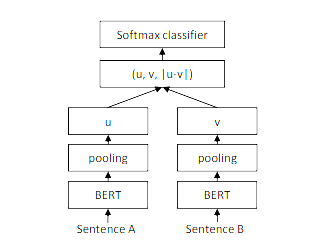
\includegraphics[width=0.7\textwidth]{styles/diploma/inc/sbert1.png} 
    \caption{Архитектура SBERT с функцией цели классификации, например, для дообучения на датасете SNLI. Две сети BERT используют общие веса (сиамская архитектура).}
    \label{fig:example}
\end{figure}


 \subsubsection{Функция цели для регрессии}. 
 
 Между двумя эмбедингами предложений}
Между двумя эмбедингами предложений $u$ и $v$ вычисляется их косинусное сходство (см. рисунок 5). В качестве целевой функции используется среднеквадратичная ошибка (mean-squared error, MSE).}


\begin{figure}[h!]
    \centering
    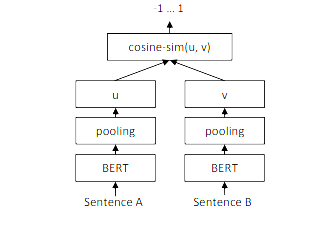
\includegraphics[width=0.7\textwidth]{styles/diploma/inc/sbert2.png} 
    \caption{Архитектура SBERT на этапе инференса, например, для вычисления коэффициентов семантического сходства между предложениями. Эта архитектура также используется с регрессионной функцией потерь.}
    \label{fig:example}
\end{figure}


  \subsubsection{Функция цели для триплетной потерь (Triplet Objective Function)}.
Имея якорное предложение 
$a$, положительное предложение $p$ и отрицательное предложение 
$n$, триплетная функция потерь настраивает сеть так, чтобы расстояние между $a$ и $p$ было меньше, чем расстояние между $a$ и $n$.

Математически, функцию потерь минимизируется следующим образом:

\begin{equation}
\max\left( \|\mathbf{s}_a - \mathbf{s}_p\| - \|\mathbf{s}_a - \mathbf{s}_n\| + \epsilon,\ 0 \right),
\end{equation}

где:
\begin{itemize}
    \item $s_x$ — эмбединги предложений $a$,$n$ или $p$;
    \item  $\|{\cdot}\|$ — метрика расстояния;
    \item  $\epsilon$ — зазор (margin).
\end{itemize}  

Значение $\epsilon$ гарантирует, что эмбединги $s_p$ находятся как минимум на $\epsilon$ ближе к $s_a$, чем $s_n$. В качестве метрики используется евклидово расстояние, и в экспериментах устанавливается $\epsilon = 1$.


 \subsubsection{Тестирование}
Результаты SBERT вместе с другими популяпными моделями, в том числе BERT.

\begin{table}[H]
\centering
\small
\caption{Скорреляции Спирмена $\rho \times 100$ для задач STS без учёта обучающих данных STS.}
\begin{tabular}{lccccccc}
\toprule
\textbf{Модель} & STS12 & STS13 & STS14 & STS15 & STS16 & STSb & SICK\textsubscript{R} & Avg.\\
\midrule
Avg. GloVe              & 55.14 & 70.66 & 59.73 & 68.25 & 63.66 & 58.02 & 53.76 & 61.32\\
Avg. BERT               & 38.78 & 57.98 & 57.98 & 63.15 & 61.06 & 46.35 & 58.40 & 54.81\\
BERT CLS                & 20.16 & 30.01 & 20.09 & 36.88 & 38.08 & 16.50 & 42.63 & 29.19\\
InferSent‐GloVe         & 52.86 & 66.75 & 62.15 & 72.77 & 66.87 & 68.03 & 65.65 & 65.01\\
USE                     & 64.49 & 67.80 & 64.61 & 76.83 & 73.18 & 74.92 & 76.69 & 71.22\\
\midrule
\textbf{SBERT-NLI-base} & 70.97 & 76.53 & 73.19 & 79.09 & 74.30 & 77.03 & 72.91 & 74.89\\
\textbf{SBERT-NLI-large}& 72.27 & 78.46 & 74.90 & 80.99 & 76.25 & 79.23 & 73.75 & 76.55\\
SRoBERTa-NLI-base       & 71.54 & 72.49 & 70.80 & 78.74 & 73.69 & 77.77 & 74.46 & 74.21\\
SRoBERTa-NLI-large      & 74.53 & 77.00 & 73.18 & 81.85 & 76.82 & 79.10 & 74.29 & 76.68\\
\bottomrule
\end{tabular}
\end{table}

\begin{table}[H]
\centering
\small
\caption{Spearman $\rho \times 100$ на тесте STSb. $\pm$ — стандартное отклонение по 10 запускам.}
\begin{tabular}{lcc}
\toprule
\textbf{Модель} &  Обучение &  $\rho$ \\
\midrule
Avg. GloVe                                  & –                      & 58.02\\
Avg. BERT                                   & –                      & 46.35\\
InferSent (GloVe)                           & –                      & 68.03\\
USE                                         & –                      & 74.92\\
\textbf{SBERT-NLI-base}                     & без STS               & 77.03\\
\textbf{SBERT-NLI-large}                    & без STS               & 79.23\\
BERT-STSb-base                              & STSb                  & $84.30\pm0.76$\\
\textbf{SBERT-STSb-base}                    & STSb                  & $84.67\pm0.19$\\
BERT-NLI-STSb-large                         & NLI+STSb              & $88.77\pm0.46$\\
\textbf{SBERT-NLI-STSb-large}               & NLI+STSb              & $86.10\pm0.13$\\
\bottomrule
\end{tabular}
\end{table}

\begin{itemize}
  \item Поиск самой похожей пары в коллекции из $10\,000$ предложений:
  \begin{itemize}
    \item \textbf{BERT} — $n(n{-}1)/2 \approx 5\times10^{7}$ сравнений $\Rightarrow$ $\sim65$ часов на V100 GPU;
    \item \textbf{SBERT} — $n$ инференсов ($\sim$5 с) + cosine-similarity ($<$0.01 с).
  \end{itemize}
  \item Тонкая настройка SBERT занимает $<20$ минут на одном GPU.
\end{itemize}


Хотя SBERT демонстрирует впечатляющие показатели качества, для конечного пользователя важна не только точность, но и время отклика системы. Чтобы снизить задержки при обработке запросов и масштабировать решение под высокую нагрузку, целесообразно развернуть модель в рамках микросервисной архитектуры: вынести SBERT-сервис в отдельный контейнер и параллелить запросы через легковесный API-шлюз. 

Таким образом возможно одновременно и сохранить высокое качество семантического поиска ,и обеспечить быстроту реакции, что критично для реальных приложений.